\documentclass[lettersize,journal]{IEEEtran}
\usepackage{amsmath,amsfonts}
\usepackage{algorithmic}
\usepackage{algorithm}
\usepackage{array}
\usepackage[caption=false,font=normalsize,labelfont=sf,textfont=sf]{subfig}
\usepackage{textcomp}
\usepackage{stfloats}
\usepackage{booktabs}%For toprule, midrule etc
\usepackage{caption}
\usepackage{url}
\usepackage{verbatim}
\usepackage{gensymb}
\usepackage{graphicx}
\usepackage{cite}

\hyphenation{op-tical net-works semi-conduc-tor IEEE-Xplore}
% updated with editorial comments 8/9/2021

\begin{document}

\title{What is the Optimal Electricity Share for Very Inexpensive Solar PV Energy?}

\author{Adam Jay Dvorak \IEEEmembership{Student, IEEE}, Marta Victoria 
        % <-this % stops a space
% \thanks{This paper was produced by the IEEE Publication Technology Group. They are in Piscataway, NJ.}% <-this % stops a space
\thanks{A.J. Dvorak and M. Victoria are with iCLIMATE Interdisciplinary Centre for Climate Change and the Mechanical and Production Engineering Department, Aarhus University, Aarhus, Denmark}
\thanks{M. Victoria is with the Novo Nordisk Foundation CO$_2$ Research Center, Aarhus, Denmark}}

% The paper headers
\markboth{IEEE Journal of Photovoltaics, November 2022}
{Adam Dvorak, Marta Victoria \MakeLowercase{\textit{et al.}}: What is the Optimal Electricity Share for Very Inexpensive Solar PV Energy?}

% \IEEEpubid{0000--0000/00\$00.00~\copyright~2021 IEEE}
% Remember, if you use this you must call \IEEEpubidadjcol in the second
% column for its text to clear the IEEEpubid mark.

\maketitle

\begin{abstract}
Solar PV is already the cheapest option to produce electricity in many world regions. Moreover, the price of utility-scale solar power plants in 2050, while highly uncertain, could decrease by over an order of magnitude from today’s costs with present-day learning rates and projected solar capacities. In this work, we analyze how this and other characteristics of solar resource affect the optimal share of electricity demand supplied by solar in different energy systems. We first use a simplified, open, hourly resolved, copper plate model for four isolated regions, with only wind and solar generation allowed, to identify the core dynamics. Using this model, we show that future cost assumptions of utility solar affect energy systems in regions with comparable strength of solar and wind resource compared to regions with much stronger solar or much stronger wind resource. Then, we use a multi-country, networked, sector-coupled  model of the European energy system (PyPSA-Eur-Sec) to analyze not only the effect of solar characteristics in a comprehensive energy system, but also how our model assumptions themselves affect the optimal share of solar. While we do not find a single variable that is determinative of the solar share of a region, we find that assumptions of system properties such as transmission or sector-coupling can greatly affect the optimal solar penetration at the country level.
\end{abstract}

\begin{IEEEkeywords}
Energy system modeling, decarbonization, green transition, PyPSA, PyPSA-Eur-Sec, sector coupling, transmission, optimization
\end{IEEEkeywords}

\section{Introduction}
\IEEEPARstart{D}{ecarbonization} by 2050 would require rapid growth of renewable technologies on a massive scale, fueled by cost reductions through research as well as improvements in the fabrication and implementation process. Solar photovoltaics (PV) is well positioned to drive this growth given its global ubiquity and status as the cheapest source of electricity in history \cite{noauthor_solar_nodate}. The cost of solar PV has decreased rapidly, dropping two orders of magnitude in the past 40 years \cite{haegel_terawatt-scale_2019}. Between now and 2050, the price could drop even further, enabling solar PV to achieve the growth required to attain timely decarbonization of energy systems.

There are many present-day indicators of the potential for future energy systems to have very high solar share, or percentage of a system's electricity demand supplied by solar PV. On the one hand, several models predict high solar share by 2050 \cite{frew_sunny_2019, breyer_role_2017, victoria_early_2020, Breyer_history, luderer_impact_2022, D1EE02497C}. On the other hand, solar share in real power systems keeps breaking records with California supplying a quarter of its electricity demand with solar PV in 2021\cite{feldman_fall_nodate} and South Australia covering 100\% of its electricity demand for one hour with rooftop solar PV \cite{parkinson_rooftop_2021}. At current prices, PV is already playing a major role in the energy systems of sunny places. If solar PV becomes cheaper, it could play a bigger role, including in places with worse solar quality. 


While it is trivial to say that the optimal solar share of a decarbonized energy system relies on the properties of solar, such as cost and resource availability, it does not solely depend on them. This is because the variability of solar must be balanced, whether by other renewable technologies, such as wind; by storage technologies, such as batteries; or by other flexibilities present in the system, such as transmission and electrification of other sectors including heating, transport, and industry. Since we do not know all the details about what these future decarbonized energy systems will look like, we modellers need to make assumptions about the system, choosing to include or exclude system properties that we think will be present. These choices may significantly affect what we try to study.

Knowing that the solar share may be affected by both solar and system properties, we investigate the following research questions: What is the optimal solar share in a decarbonized energy system? What are the main factors that impact it? How do our model assumptions affect our results?

We begin this investigation by looking at simple representations of real energy systems based in regions with different wind and solar resource. Each region is limited to solar and wind generators. We do not include any fuel-based generators because we model scenarios with zero CO$_2$ emissions. Additionally, we do not include hydropower or run of river in our model. Only battery and hydrogen storage are available for balancing. Using simplicity is an intentional choice: by only using the minimum required elements to model the fluctuations in wind, solar, and electricity demand, we can easily and clearly get to core dynamics that affect solar share. We select a “warm” region and a “cold” region in the United States, California (CA) and Colorado (CO); and in Europe, Spain (ESP) and Denmark (DNK). While California is not a perfect analog to Spain and Colorado is not a perfect analog to Denmark, there is significant enough variation between the four regions to begin an analysis into core dynamics. See the main seasonal patterns in Fig. 1. 



Using this simple model, we analyze the impact of the following parameters: cost assumptions for solar PV, wind, and battery; increasing or decreasing the carbon allowance; and electrifying heating. Although many modelled scenarios with high penetration of solar exist \cite{victoria_early_2020, Bogdanov2019, CHILD201980, JACOBSON2017108}, one novelty of this paper is that we focus on unveiling what determines the optimal solar share. We even assume the cost of solar PV to become extremely cheap due to learning, as an academic exercise. See Section 3.1 for details.


Of course, energy systems in reality are much more complex than a single node with solar and wind generators. There are other types of electricity generators, and there are more uses of energy besides electricity. Local energy systems are connected as part of broader systems. These additional complexities could affect the optimal solar share. To capture some of these complexities, we turn to an open, sector-coupled model of Europe, PyPSA-Eur-Sec\cite{pypsa_eur_sec, victoria_speed_2022}. Using PyPSA-Eur-Sec, we investigate how latitude, solar quality, and wind quality affect solar share, and analyze how their effect changes between different models, such as coupling electricity with other sectors (heating, transportation, industry),  or including transmission lines that interconnect countries. Investigating how system properties interact with these critical input variables is the main novelty of this paper.




\section{Methods}
\subsection{Single-node simplified model}
For our simple model, we use Python for Power System Analysis (PyPSA) \cite{brown_pypsa_2018} to model the power system. We determine the optimal capacity and dispatch of wind and solar PV generators that minimize the system cost while supplying uninterrupted hourly demand for a full year. We investigate four regions: Colorado (CO), California (CA), Denmark (DNK), and Spain (ESP). For each region, we assume a single-node, copper-plate model. We assume generators of solar and wind, battery and hydrogen storage, and zero CO$_2$ emissions. Baseline prices in 2020 are shown in Table \ref{costs}.


\begin{center}

\begin{tabular}{llll}
\toprule
Technology & Cost & Efficiency & Lifetime(yrs) \\
\midrule
Utility Solar        &      529 €/kW   & -  &   35  \\
Onshore wind         &     1118  €/kW  & -   &   27  \\
Battery storage         &     232 €/kWh   & - &  20  \\
Battery inverter          &     270 €/kW & 0.95 & 10   \\
$H_{2}$ storage        &     3.0  €/kWh & - &   100  \\
Fuel cell &           1300 €/kW   &    0.5  &    10  \\
Electrolysis &           650 €/kW  & 0.66  &  25  \\
\bottomrule
\end{tabular}
\captionof{table}{Table of costs in 2020 for technologies used with PyPSA, given in 2015 money. Costs, efficiencies, and lifetimes are taken from\cite{danishreport}. Discount rate is 7\% for all technologies. The one-way efficiency for the battery inverter is listed. H$_2$ storage is assumed to be underground salt caverns. }\label{costs} 

\end{center}

We use electricity demand from 2011 from \cite{welty_ethan_US_ED} for CO and CA as well as electricity demand from 2015 from ENTSOE for DNK and ESP \cite{entsoe_timeseries}. Capacity factors (CFs) for solar and wind are obtained from the following repositories for DNK and ESP\cite{victoria_PV_timeseries, victoria_wind_timeseries}, and from  renewables.ninja \cite{renewableninja, STAFFELL20161224, PFENNINGER20161251} for CO and CA. The electricity demand and CFs are plotted over the course of the year in Figure \ref{fig: ED_CF_all}, with the average CF listed on the right hand side for solar and wind. Seasonal patterns are strong in some regions (DNK) but not as dominant in others.

\begin{figure}[H]
\centering
\includegraphics[width=1\linewidth]{Figures/updatedSeasonalVars.png}
\caption{Weekly solar and wind resources and electricity demand over the course of the year for the four regions normalized to the average. The average wind/solar CFs for each region are to the right of the respective plot, in blue/orange.} 
\label{fig: ED_CF_all} 
\end{figure}



\begin{figure}[H]
\centering
\includegraphics[width=1\linewidth]{Figures/elecdem_newplot.png}
%\includegraphics[width=\textwidth]{figure_name.png}
\caption{Weekly average of electricity demand by temperature is plotted for a historical weather year (2015 for DNK and ESP, 2011 for CA and CO)} 
\label{fig: electempall} 
\end{figure}


It is clear that there is a relationship between a country's electricity demand and temperature. In Figure \ref{fig: electempall}, we observe that a profile of a given country's electricity demand vs temperature can have up to three distinct regions--a negative correlation between electricity demand and temperature, a positive correlation, or a correlation with a slope of 0. We find that these three regions begin or end at a temperature threshold $T_{th}$, which varies by country.



We performed two simulations: one with the demand timeseries as shown in Figure \ref{fig: electempall}, and one with the coupled electricity and heating system. In a system with zero carbon emissions, we assume that all heating demand is electrified, using heat pumps with a coefficient of performance of 3. To calculate the heating demand, we follow Victoria et al. \cite{victoria_storage_2019}, separating demand into a constant water heating $HD_{water}$and a variable space heating proportional to the difference between the ambient temperature $T_{amb}$ and $T_{th}$, chosen to be 17\degree C. This is the number of Heating Degree Hours (HDH). For a given time step, the total heating demand ($HD_{tot}$) is given by eq. \ref{eq: HD}

\begin{equation}
    HD_{tot} = \sum G (T_{th} - T_{amb}) + HD_{water}
    \label{eq: HD}
\end{equation}

where $G$ is the coefficient, unique to each region, of how much heating demand is added per HDH. 

We use heating data from Victoria et al. for Denmark and Spain. We need to calculate heating demand for CA and CO. First, we use temperature series from renewables.ninja\cite{renewableninja, STAFFELL20161224, PFENNINGER20161251} to calculate the HDH for CA and CO and scale the timeseries to match the annual energy demand for space heating \cite{EIA_dataset}. From this dataset, we have space heating and water heating for households in each state. To estimate the total heating demand, we assume that the percentage of household heating demand of the total is the same as that of the electricity demand. We find $G$ to be 1715 and 1782 (MWh/HDH) for CA and CO, respectively. 

When adding this calculated heat demand to the electricity demand, we get the demand series in Figure \ref{fig: tempincreaseall}. For each of the analyses of solar, wind, and battery cost in the results section, we plot the results from both demand time series in this figure. 

\subsection{Networked sector-coupled model}
For the fully detailed model, we use an open, sector-coupled model PyPSA-Eur-Sec \cite{pypsa_eur_sec}. We model with 37 nodes across 33 countries and 3-hourly resolution for an entire year.  More info about PyPSA-Eur-Sec can be found from Victoria et. al \cite{victoria_speed_2022} and the website \cite{readthedocs}.

\begin{figure}[H]
\centering
\includegraphics[width=1\linewidth]{Figures/elecheatdem_temp_newplot.png}
%\includegraphics[width=\textwidth]{figure_name.png}
\caption{Weekly average of electricity demand, assuming electrified heating demand, is plotted by temperature for a historical weather year (2015 for DNK and ESP, 2011 for CA and CO). The modified values are overlayed on top of Figure \ref{fig: electempall}. }
\label{fig: tempincreaseall} 
\end{figure}


\section{Results--Single Node Simplified Model} 

\subsection{Sensitivity to cost of Solar}
Since we optimize the system cost, we expect the cost of solar PV to directly affect the optimal solar share. Europe has the goal of achieving carbon neutrality by 2050 \cite{Europe_climate_goal}, so we project solar PV costs to this timeframe.

We project the cost of utility solar PV by using the learning rate, which is the percent decrease in cost per doubling of cumulative capacity. The learning rate of utility solar PV has historically been 23\%, but has more recently reached 40\% \cite{victoria_solar_2021}.  Haegel et al. projects 
cumulative global capacity of solar PV to reach 30-70 TW by 2050 \cite{haegel_terawatt-scale_2019}. The global capacity of solar PV in 2020 was 770 GW \cite{IEA_snapshot_2020}, meaning that by 2050, the capacity of solar PV would have doubled between 5.3 and 6.5 times. The price of utility scale solar PV in 2020 can be estimated to be 0.529 \texteuro/Wp \cite{IEA_snapshot_2020}, but can also reach up to 1.3 \texteuro/Wp \cite{vimmerstedt_2021_2021}. The cost of solar PV is known to vary widely by region \cite{IRENA}.

We generate a range of projected utility solar PV costs by extrapolating with these learning rates and capacity projections from the 2020 price of 0.529 \texteuro/Wp and 2020 capacity of 770 GW. If we take the least optimistic scenario, with a learning rate of 23\% and only 30 TW installed, that would correspond with a price of 0.132 \texteuro/Wp for utility solar PV, or about four times cheaper than the 2020 price. If we were to take the most optimistic scenario, with 70 TW installed and a learning rate of 40\%, we would expect a price of 0.019 \texteuro/Wp, over an order of magnitude cheaper than the 2020 price. We can then compare ``less optimistic” and ``optimistic” scenarios. We acknowledge that the ``optimistic” scenario may be more optimistic than realistic, considering that we assume the learning rate of solar modules to be that of the entire PV system. In addition, even with a high learning rate, there may be costs associated with grid and land usage that are non-negligible. Nevertheless, we plot values up to 0.01 \texteuro/Wp as an academic exercise to better understand what would happen in a universe with extremely cheap solar.







\begin{figure}[H]
\centering
\includegraphics[width=1\linewidth]{Figures/Figure3_solar_sensitivity_w_and_woHeat_ver_13_10_2022.png}
%\includegraphics[width=\textwidth]{figure_name.png}
\caption{Electricity mix and curtailment of solar is plotted for the four regions of study, with solar cost in €/Wp on the x-axis (log scale). The opaque region shows the change that would occur if the electricity demand changes in the manner illustrated in Figure \ref{fig: tempincreaseall}} 
\label{fig: solar_temp_cooling} 
\end{figure}

In Figure \ref{fig: solar_temp_cooling}, we plot electricity mix on the y-axis and vary solar cost on the x-axis on a logarithmic scale, marking the “less optimistic” and “optimistic” price points in 2050, and the cost-range of solar of 2020. In addition, we plot the percent of solar energy that is curtailed. The ideal proportion of solar varies by region. For DNK, there is never a scenario in which 100\% solar energy is realized, whereas CA experiences 100\% solar energy at a cost similar to today's.  It makes sense for these regions to be at the two extremes of our analysis: according to Figure \ref{fig: ED_CF_all}, DNK has the highest ratio of wind to solar CF, and CA has the lowest. For CO and ESP, regions with ratios in between that of CA and DNK, we see that even lowering the cost to the “less optimistic scenario” makes a big difference for the optimal solar share. One hypothesis is that regions with moderate solar potential stand to benefit more from a decrease in solar price compared to those with high or low solar potential. However, the solar CF alone is not enough to explain our results, as CA and CO are shown to have the same average solar CF in Figure \ref{fig: ED_CF_all}.  Another hypothesis is that ESP and CO have relatively strong sources of wind and solar in comparison with DNK and CA. For ESP and CO, the model has a more balanced choice implementing solar and wind, so cost reductions in solar help tip that balance. 

We see that solar curtailment increases significantly as the price of solar decreases, approaching near-100\% of produced energy curtailed. This implies an unrealistic amount of solar installation, with capacities many times greater than the average energy system demand. We note that nothing changes dramatically when the electrified heating is added to the demand time series.

We also see that adding heating demand to the electricity load depresses the solar share, particularly in Denmark and Colorado. It makes sense that these two regions are most affected, as they have the most modification to their load as shown in Figure \ref{fig: tempincreaseall}. As one would expect the seasonality of solar to be anti-correlated with the seasonality of heating, the fact that solar share is depressed also makes sense. However, the overall trend still holds--there is still a great benefit to solar share between today's range and the future range for all regions.

\section{Results: Networked Sector-Coupled Model of Europe}

To help better identify variables that determine solar quality, we turn to PyPSA-Eur-Sec. PyPSA-Eur Sec\cite{pypsa_eur_sec} allows us to capture complex dynamics of 33 interconnected European countries as a representation of the real European energy system. With a more realistic model and more regions to investigate, we try to better understand the effect of three fundamental variables that may influence the solar quality: latitude, solar CF, and wind CF. Since the computational power required to solve one configuration of PyPSA-Eur-Sec is many orders of magnitude larger than solving one node of PyPSA,  we will only look at three costs: today's cost of solar PV, the ``optimistic" cost, and the ``less optimistic" cost, as presented earlier.

While analyzing latitude should be similar to analyzing the solar CF, it is still worthwhile to do this separate analysis. The regional variation of climate means that different countries at the same latitude may not have the same solar CF, whereas the latitude of a country will not change between different model runs. In addition, latitude can provide a visual intuition as to how patterns change.


Another focus of this paper is to identify how changes in the system itself affect solar quality. Each experiment also compares how the solar share is affected by the presence of  transmission between nodes, and/or the inclusion of other sectors besides electricity, such as industry and heating. This gives us four completely different systems: one with transmission and sector-coupling, one each with either transmission or sector-coupling, and one with neither transmission nor sector-coupling. For each system, we plot the variable of investigation on the x-axis and the solar share on the y-axis for each of the 33 countries. From this, we plot a line of best fit, and analyze the goodness of fit using the coefficient of determination $r^{2}$.


\subsection{Latitude}



We first investigate the effect of latitude by plotting the solar share for the four systems on a map of Europe, in Figure \ref{fig: europemaplats}. The plotted solar share is from the "less optimistic" solar cost, which corresponds to one quarter the price of today. 

\begin{figure}[H]
\centering
\includegraphics[width=1\linewidth]{Figures/solarlatmap.png}

\caption{A map of Europe is used to graphically illustrate how latitude affects solar penetration, and how adding either sectors or transmission changes this dynamic. The overall solar share is in red text at the upper left of each plot. Note: Kosovo is not included in the PyPSA-Eur-Sec model and has no data.} 
\label{fig: europemaplats} 
\end{figure}

Visually, one can see that there is more solar overall when sectors are added. The main reason is that when coupling the transport sector, the system includes electric vehicle (EV) batteries which behave similarly to static batteries, encouraging high shares of solar PV, as shown in Figure \ref{fig: solar_batt}. Conversely, adding transmission decreases solar share. Transmission is known to balance wind better than solar because wind has a shorter correlation length, meaning that it can reap more benefits from spatial smoothing of power generation \cite{victoria_role_2020}. The effect of sector-coupling on solar penetration has also been previously shown by Victoria et. al (2020) \cite{victoria_role_2020}. 



In addition to decreasing the overall solar penetration, transmission is shown to decrease the correlation of solar share with latitude. For example, in the system with transmission and without sectors, Portugal has much less solar than its neighbor, Spain, even though they are roughly at the same latitude. The system optimizes for Spain to use solar and Portugal to use something else, such as hydro or wind, because Spain has a higher solar capacity factor than Portugal.

We can see this effect more clearly in Figure \ref{fig: solar_by_lat}, where we plot the solar penetration by country, with countries ordered by latitude on the x-axis, increasing. The implied values in Figure \ref{fig: europemaplats} are the same as the red dots in Figure \ref{fig: solar_by_lat}, where the cost of solar is 25\% of today’s cost, or the ``less optimistic" cost for 2050. Both Figures \ref{fig: europemaplats} and \ref{fig: solar_by_lat} show that the correlation of solar with latitude is disturbed when adding transmission. By contrast, adding sectors to a system restores and strengthens correlation. 

\begin{figure}[H]
\centering
\includegraphics[width=1\linewidth]{Figures/fourlatitude_compare.png}

\caption{The solar penetration for each country is plotted at the prices of today's, "less-optimistic", and "optimistic" levels. Countries are ordered on the x-axis by latitude. Due to plotting order, if any of the red dots are not visible, they can be assumed to be under the yellow dots for the respective country} 
\label{fig: solar_by_lat} 
\end{figure}

Like the single-nodal model, we see that cost reductions of solar affect regions differently. In seven countries (ES, RO, SI, FR, HU, CZ, IE), half of the electricity supply transforms into solar PV when the cost of solar decreases from ``less optimistic" to ``optimistic", showing high sensitivity to cost like the regions CO and ES. Other countries are already saturated, whereas some countries are minimally affected. One consequence of transmission is that cost reductions of solar can actually decrease solar penetration locally. This occurs in the system with transmission and no sectors in Figure \ref{fig: solar_by_lat} in the countries of Croatia (HR), Montenegro (MK), Switzerland (CH), and Luxembourg (LU). When taking into account both global and local incentives, this strange phenomenon can make sense. Lowering the cost of solar may cause countries with a comparative advantage in solar PV to further exploit their advantage, allowing their neighbors to invest in other resources.





\subsection{Average solar quality}
We expect there to be a positive correlation between the solar CF and the solar penetration. In Figure \ref{fig: solar_by_solarcf}, we plot results from PyPSA-Eur-Sec for each country to see the strength of this correlation in the four different systems.


\begin{figure}[H]
\centering
\includegraphics[width=1\linewidth]{Figures/cap_factor_solar.png}

\caption{ Percent of electricity generated by solar is plotted vs. the average solar CF. The coefficient of determination between the two variables r$^2$ is shown for each plot. } 
\label{fig: solar_by_solarcf} 
\end{figure}

While there is a positive correlation between the solar CF and solar penetration in all systems, the strength of the correlation depends on the type of system that we use. For the system with neither sector-coupling nor transmission there is weak correlation. With no other balancing available, the variability in other renewable resources, such as wind, hydro, or run of river, may matter more in the balancing of a single node. In contrast, sector-coupling increases correlation. This was seen previously with latitude, and may also be explained by the better correlation due to EVs.





\subsection{Average wind quality}

Wind and solar PV are competing generators, so we expect a negative correlation between the amount of solar generated in a system and the wind CF. This is indeed what we find in Figure \ref{fig: solar_by_windcf}.


\begin{figure}[H]
\centering
\includegraphics[width=1\linewidth]{Figures/cap_wind_paper.png}

\caption{ Percent of electricity generated by solar is plotted vs. the average wind CF of each country.  The coefficient of determination between the two variables r$^2$ is shown for each plot.} 
\label{fig: solar_by_windcf} 
\end{figure}

Interestingly, the correlation of the wind CF with solar share, while negative, is stronger than that of solar CF with solar share. This implies that the optimal amount of solar installed in a system is as dependent on the wind quality of a region as the solar quality of a region, or more so. This could help explain why the simple model shows CA to be so solar dominated and CO to be more balanced--it is not that CA has better solar than CO, but worse wind. 


\section{Discussion}

Throughout this paper, we have not been able to come up with a single variable or method to find the optimal solar penetration in an energy system. This is because we have shown that the optimal value of solar for a region is not only sensitive to its own unique time series of solar and wind, but also to the properties of the system--for example, when transmission is expanded, a country such as Portugal can completely flip from a major solar producing country to a minor one. The solar share by country is shown to be correlated with regional variables such as CF, but with no $r^2$ value greater than 0.6, we show that no variable is singularly determinative of the solar PV share. In addition, important variables such as the cost of relevant systems in 2050 (PV, wind, battery) are hard to predict, with varying expert predictions and high historical learning rates. Yet, we show that the optimal amount of solar PV is highly dependent on these costs for many regions. 

At the same time, this study also shows that some regions have more to gain from reductions in utility solar PV cost compared to others. We do not need solar PV cost reductions to perform at historical learning rates--for many places, a moderate cost reduction would still create vast system changes. On the other hand, many places do not stand to gain as much from reducing solar cost due to saturation of solar or weak solar resource. For example, in both the simple and fully-resolved models, we show Denmark is always heavily dependent on wind, regardless of the cost of solar or battery. In contrast, we found Spain to be heavily dependent on both the cost of solar and the cost of battery.

It is important to note some of this study's many limitations. This study lacks sensitivity studies to the reliance on results to time nor space resolution. Additionally, our inclusion of sector-coupling and/or transmission is a purely binary choice. In reality, a decarbonized future energy system would have some form of both sector-coupling and transmission, but our analysis does not go beyond or below the default inclusion. This analysis focuses on the European energy system. To completely analyze factors that affect solar penetration, it would be helpful to model energy systems in regions closer to the equator, as these are the places that are likely to implement the most solar. These regions would generally use more energy for cooling and less for heating compared to Europe--it would be interesting to see the impact of increased cooling demand for these systems because of the natural correlation with solar PV, especially for a warming world.\cite{laine_meeting_2019, zhu_impact_2020}

Future studies investigating how properties of solar and the system itself affect the solar share may continue analysis with PyPSA-Eur-Sec and perform a more detailed cost-sensitivity analysis. This would help to determine if there are threshold costs for each given scenario at which a decrease in solar cost becomes less beneficial. In addition, a future study involving a parameter sweep of the CO$_2$ limit would be helpful to determine the point at which saturation of solar in CA and other regions is no longer an issue. Finally, parameter sweeps of multiple variables at once, e.g. using Monte Carlo simulations, may be helpful to explore more realistic scenarios where multiple technologies are benefiting from learning.


\section{Conclusion}
This paper attempted to find factors that influence the optimal solar share within an energy system. We did this by starting with a simple one-node capacity and dispatch optimization model for four regions (Denmark, Spain, California, Colorado) and running parameter sweeps of cost of solar, wind, and battery, with and without the assumption of electrified heating. We found that in regions with strong solar and wind (CO, ESP), cost reductions for one or the other can heavily tilt the playing field in favor of one technology. On the other hand, regions with weak wind or weak solar (DNK, CA) do not experience the same gains. Using a networked, sector-coupled model of Europe, we compared systems with and without transmission and sector-coupling. In line with other literature, we found that sector-coupling is beneficial for solar penetration while transmission has the opposite effect. We also found that transmission can make the system behave nonintuitively, disturbing the expected correlation between latitude and solar penetration, because neighbors of countries with stronger solar resource can instead focus on different energy sources, even as solar gets cheaper overall. We were unable to find a single determinative variable of the optimal solar share of a region, as this is a result of complex interactions among different components of a system.


\section*{Acknowledgments}
A.D. is fully funded by Fulbright Denmark. M.V. acknowledges funding from European Union’s Horizon 2020 program (AURORA project under grant agreement no. 101036418).



\bibliographystyle{IEEEtran}
\bibliography{bib_high_solar_penetration}



\newpage

\section{Biographies}

 



\begin{IEEEbiographynophoto}{Adam Jay Dvorak}
Originally hailing from Santa Rosa, CA, Adam Dvorak completed his BA in physics from Pomona College in 2021. After receiving a 2021 U.S. Fulbright Scholarship to Denmark, he embarked on a journey across the ocean to start working with Professor Marta Victoria on the decarbonization of energy systems at Aarhus University, Denmark. He is currently working on incorporating biomethanation as a green source of methane in energy systems. In his spare time, he likes to play violin, sing in his barbershop chorus, and play board games.
\end{IEEEbiographynophoto}

\vspace{11pt}

\begin{IEEEbiographynophoto}{Marta Victoria}
Marta Victoria received the B.Sc. and M.Sc. degrees in aerospace engineering from the Technical University of Madrid and a PhD degree in high-efficiency photovoltaic modules from the Solar Energy Institute, Technical University of Madrid. She is an Associate Professor at the Department of Mechanical and Production Engineering, Aarhus University, Denmark. Her research focuses on the modelling of large-scale energy systems with high renewable penetration paying special attention to the role of solar photovoltaics. She is a member of the Open Energy Modelling Initiative, which aims to promote openness and transparency in energy systems modelling, and she co-develops the open-source energy model PyPSA-Eur-Sec.
\end{IEEEbiographynophoto}



\vfill

\end{document}


